\clearpage
\section{Representere et system med ligninger}\label{sec:massetransport}


Når vi snakker om å representere et system med ligninger mener vi å sette opp balanseligninger. I prossmod er det et fåtall av ligninger du trenger å kunne, men en av de viktigste er hvordan vi setter opp en balanse for et lumped system/kontrollvolum.
\begin{equation}
    \label{eq:akkumulering_generell}
    Akkumulering = Inn - Ut + Generert 
\end{equation}

Kort fortalt ønsker vi å sette opp en ligning for hvordan en ekstensiv variabel endrer seg inne i volumet. Fra \cref{eq:akkumulering_generell} ser vi at endringen inne i volumet er avhengig av transporten inn og ut, og hvor mye som genereres/forbrukes inni volumet. Merk at vi bare kan sette opp en slik balanse for ekstensive variabler siden intensive variabler er uavhengig av størrelsen på systemet. Vi bruker variabelen $\Phi$ som en vilkårlig ekstensiv variabel videre i kapittelet.  

\subsection{Balanser og konservering}\label{sec:balanser_konservering}
\begin{align} \label{eq:konservering_generell}
    \text{Konservering: }\dot{\Phi}_{system} &= \hat{\Phi}_{inn} - \hat{\Phi}_{ut} \\
    \label{eq:balanse_generell}
    \text{Balanse: }\dot{\Phi}_{system} &= \hat{\Phi}_{inn} - \hat{\Phi}_{ut} + \Tilde{\Phi}_{system}
\end{align}

En konservering er en balanse hvor genereringen av den ekstensive variabelen er null, dvs. all akkumulering skyldes transport inn og ut av systemet. Et system kan ofte bestå av balanser og konserveringer. For eksempel i en reaktor vil det genereres stoffmengde, men den totale massen vil være konservert.  Du kommer deg fint gjennom livet ved bare å bruke terminologien balanser, men vær klar over at en balanse blir en konservering når det ikke er generering/forbruk, det vil si $\Tilde{\Phi}_{system}$ = 0. For å ikke forvirre leseren vil vi bruke terminologien balanse videre i kompendiet.

\subsection{Sette opp en enkel balanse fra en topologi} \label{sec:balanse_enkel}

\begin{figure}[H]
    \centering
    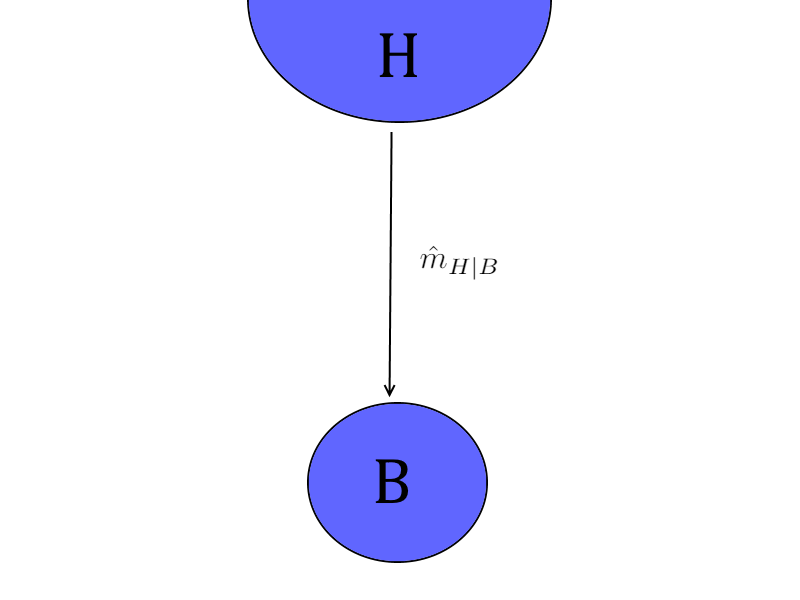
\includegraphics[scale=0.3]{Figures/Basseng1.png}
    \caption{Topologi av regnvann inn i et basseng, H representere himmel og B representerer bassenget.}
    \label{fig:topologi_enkel2}
\end{figure}
Det er kun rundt systemer med kapasitet vi kan gjøre balanser (lumped/distributed). I vår topologi, gitt i \cref{fig:topologi_enkel2}, er H et reservoar og er ikke interessant å gjøre en balanse rundt siden kapasiteten er uendelig ($\dot{\Phi}_H=0$). Volumet B kan vi sette opp en balanse rundt ved å bruke \cref{eq:balanse_generell}:

\begin{equation}
    \dot{\Phi}_{B} = \hat{\Phi}_{H|B}
\end{equation}

Vi vet alt at vår ekstensive variabel fra topologien er masse så kan vi bytte ut $\Phi$ med $m$:


\begin{equation}
    \dot{m}_B = \hat{m}_{H|B}    
\end{equation}
Vi har nå en ligning for systemet vårt og vi kan regne ut akkumuleringen av masse i B hvis vi vet transporten fra H til B. 

\subsection{Eksempel: Sette opp balanser for flere systemer}\label{sec:flere_massebalanser}
\begin{figure}[H]
    \centering
    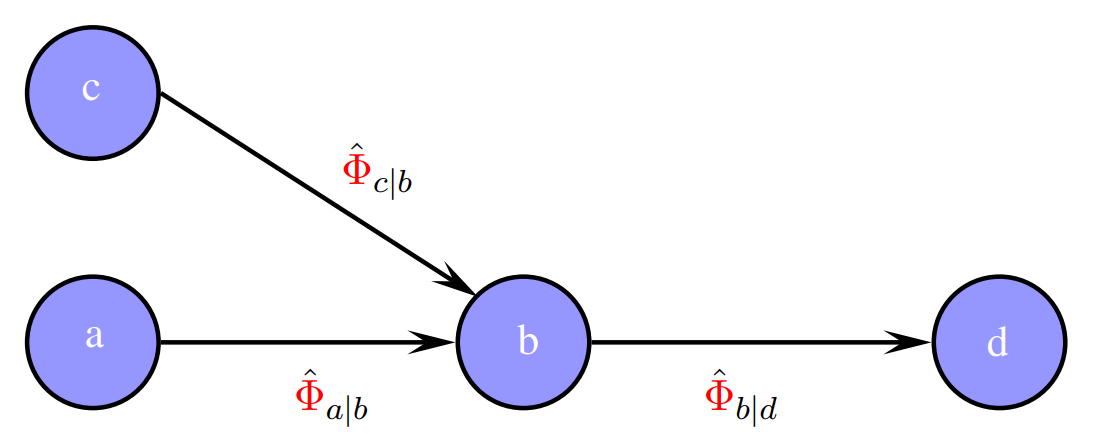
\includegraphics[scale=0.3]{Figures/massebalanser_flere_systemer}
    \caption{Topologi av fire lumped systems med transport av en ekstensiv variabel. Figur hentet fra ABC-heftet.}
    \label{fig:massebalanser_flersystem}
\end{figure}
Vi har et system bestående av fire lumped systems. Ved å benytte oss av samme teknikk som i kapittel \ref{sec:balanse_enkel} setter vi opp fire balanser: 
\begin{equation} 
    \begin{split}
    \label{eq:massebalanser_vanskelig1}
    \dot{\Phi}_{a} = & -\hat{\Phi}_{a|b} \\
    \dot{\Phi}_{b} = &\hspace{0.1cm} \hat{\Phi}_{a|b} + \hat{\Phi}_{c|b}-\hat{\Phi}_{b|d}\\
    \dot{\Phi}_{c} = & -\hat{\Phi}_{c|b}\\
    \dot{\Phi}_{d} = & \hspace{0.1cm}\hat{\Phi}_{b|d} \end{split}
\end{equation}


\subsection{Incidence matrix}
I modellering får vi ofte et system som består av flere titalls mindre systemer som gjør det vanskelig å holde styr på alle balansene. Det er derfor ønskelig å benytte seg av vektorer og matriser. 

Ved utgangspunkt i (likningssett) \ref{eq:massebalanser_vanskelig1} definerer vi vektoren for akkumulering og transport:\\ 
\begin{center}
    Vektor for akkumulering: $\underline{\dot{\Phi}}$ =
$[\dot{\Phi}_a,\dot{\Phi}_b,\dot{\Phi}_c,\dot{\Phi}_d]$ \\
Vektor for transport:  $\underline{\hat{\Phi}}$ =
$[\hat{\Phi}_{a|b},\hat{\Phi}_{c|b},\hat{\Phi}_{b|d}]$
    
\end{center}

Vi bruker disse vektorene til å representere balansene fra (likningssett) \ref{eq:massebalanser_vanskelig1} i en samlet matrise som har navn \textit{Incidence Matrix}.

\begin{equation}
    \textbf{\doubleunderline{F}} = 
    \bordermatrix{~ & \hat{\Phi}_{a|b} & \hat{\Phi}_{c|b}  & \hat{\Phi}_{b|d} \cr
                  \dot{\Phi}_a & -1 & 0 & 0 \cr
                  \dot{\Phi}_b & +1 & +1 & -1\cr
                  \dot{\Phi}_c & 0 & -1 & 0\cr
                  \dot{\Phi}_d & 0 & 0 & +1
                  }
\end{equation}
Hver rad i incidence matrix representerer en balanse og hver kolonne representerer transport fra et volum til et annet. Ved å sette opp incidence matrix kan vi skrive likningsettet \ref{eq:massebalanser_vanskelig1} som:

\begin{equation}
   \underline{\dot{\Phi}} = \textbf{\doubleunderline{F}}\hspace{0.1cm}\underline{\hat{\Phi}}
\end{equation}

Her har vi nå satt sammen et likningsett inn til en ligning med vektorer og matriser. Senere i kompendiet vil vi fortsette med denne notasjonen for å vise den lineære algebraen som kommer fram når vi modellerer. Bakgrunnen for å bruke denne notasjonen fremfor å forklare det med likninger er fordi lineær algebra har strengere krav for operasjoner enn operasjoner på skalarer i en enkel likning. Hvis du nå tenker ``Men jeg husker ikke så mye fra Matte 3'', sorry brah! Lineær algebra kommer du deg ikke utenom på IKP. Likevel, hvis du føler det er vanskelig å forholde seg til notasjonen så kan det hjelpe å skrive ut matrisen til et sett med ligninger og forholde seg til dem istedet. 

\clearpage
\subsection{Blokkmatriser}
Når man skal sette opp en incidence matrix for flere komponenter, e.g. stoffmengder, kan det være lurt å bruke matrisen til å sette opp en blokkmatrise. Dette er vanlig når man har flere komponenter som beveger seg mellom forskjellige volum. 

\begin{figure}[H]
    \centering
    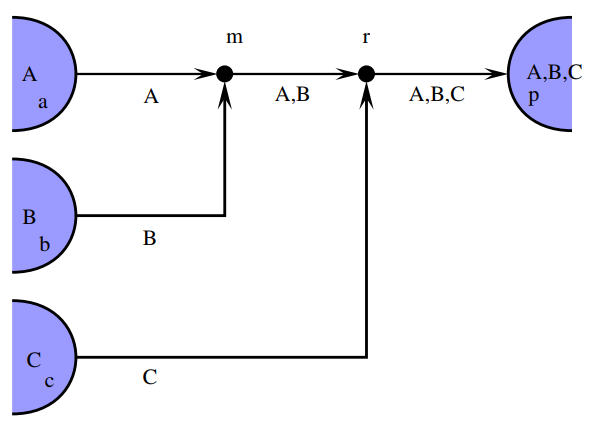
\includegraphics[scale=0.7]{Figures/Block_matrix_topo}
    \caption{Topologi av system m og r som transporerer stoffene A,B og C. Figur hentet fra ABC-heftet.}
    \label{fig:block_matrix1}
\end{figure}

\begin{figure}[H]
    \centering
    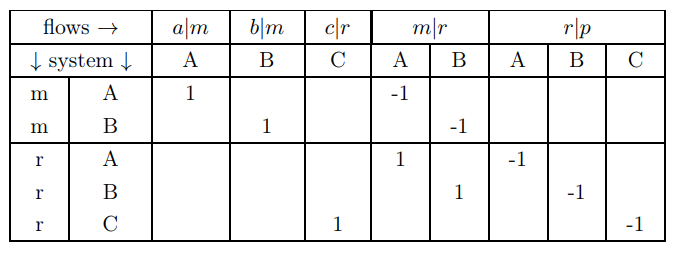
\includegraphics[scale=0.7]{Figures/Block_matrix}
    \caption{Incidence block matrix for topologien presentert i  \cref{fig:block_matrix1}. Figur hentet fra ABC-heftet.}
    \label{fig:block_marix}
\end{figure}
Vi dekker ikke denne delen i kompendiet siden prinsippet er mye av det samme, men oppfordrer sterkt å lese kapittel 7.1 i ABC-heftet hvis du ikke forstår deg på blokkmatriser.
